\documentclass[12pt,a4paper]{article}
\usepackage[margin=1in]{geometry}
\usepackage[utf8]{inputenc}
\usepackage{amsmath}
\usepackage{amsfonts}
\usepackage{amssymb}
\usepackage{graphicx}
\usepackage{enumerate}
\usepackage{bm}
\usepackage{pythonhighlight}
\usepackage{fontspec}
\usepackage{xeCJK}
\setCJKmainfont{SimSun}
\usepackage{tikz}
\usetikzlibrary{arrows,positioning}
\usepackage{float}

\geometry{left=1.00in,right=1.00in,top=1.00in,bottom=1.00in}

\title{homework 2}
\author{Zuyao Chen 201728008629002}
\date{}
\begin{document}
\maketitle
\section{Problem 1}
\qquad 对于多类情况$1$,$M$类需要$M$个判别函数;多类情况$2$,$M$类需要$M(M-1)/2$个判别函数,因此所需判别函数的最少数目为
\[
	3 + 7*(7-1)/2 = 24
\]
\section{Problem 2}
\[
	d_1(x) = -x_1, d_2(x) = x_1 + x_2 - 1, d_3(x) = x_1 - x_2 -1
\]
\begin{enumerate}[1.]
	\item 多类模式1, 下图中白色区域表示不确定性区域
	 \begin{figure}[H]
	 	\centering 
		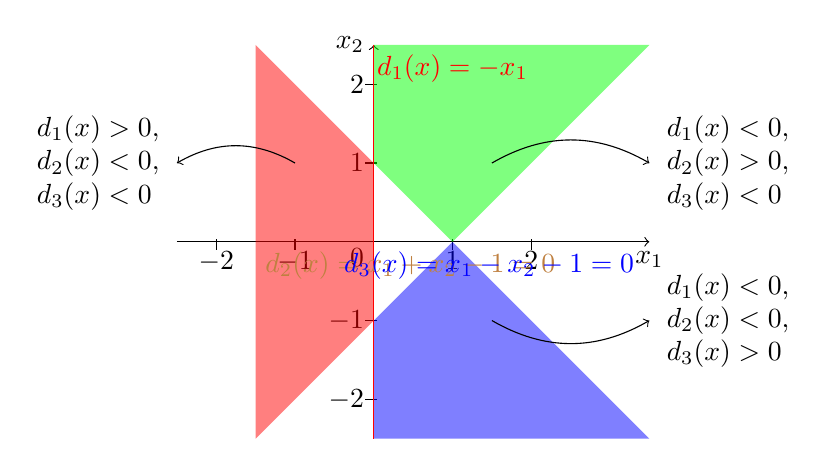
\begin{tikzpicture}  
			%axis
 		   \draw[->] (-2.5,0) -- (3.5,0) node[below] {$x_1$};
 		   \draw[->] (0,-2.5) -- (0,2.5) node[left] {$x_2$};
		   %ticks
		   \foreach \x in {-2,-1,1,2}
			   \draw (\x, 1pt) -- (\x, -3pt)
			   node[below] at (\x,0) {$\x$};
		   \foreach \y in {-2,-1,1,2}	
			   \draw (1pt,\y) -- (-3pt,\y)
	 		    node [left]at (0,\y) {$\y$}; 
	 		\node [left,yshift = -0.2cm] at(0,0) {$0$};   
		   %color
		   \fill[color = green, fill opacity = 0.5] (0,1) -- (0,2.5) -- (3.5,2.5) -- (1,0) --cycle;
		   \fill[color = blue, fill opacity = 0.5] (0,-1)-- (1,0) -- (3.5,-2.5) -- (0,-2.5) --cycle;
		   \fill[color = red, fill opacity = 0.5] (0,-1)-- (0,1)-- (-1.5,2.5) -- (-1.5,-2.5) --cycle;	 		 
		   %draw functions 
			%d1
		   \draw[color = red] (0,-2.5) -- (0,2.5) ;	
		   \node[color = red] at (1,2.2) {$d_1(x) = -x_1$ };  
			%d2
		   \draw[color = brown,domain = -1.5:3.5] plot[id = x] function{1 - x}
		   node[below right,xshift = -1.5cm] {$d_2(x) = x_1 + x_2 - 1 = 0$};
		    %d3
		   \draw[color = blue, domain = -1.5:3.5] plot[id = x] function{x-1} 
		   node[below right,xshift = -0.5cm ] {$d_3(x) = x_1 - x_2 -1 = 0$};	
			%
		   \path[->] (1.5,1) edge [bend left] node [right] {} (3.5,1);
		   \node [align = left] at (4.5,1) { 
		   	$ d_1(x) < 0$,\\$d_2(x) > 0$,\\$ d_3(x) < 0 $};
		   \path[->] (1.5, -1) edge [bend right] node [right] {} (3.5,-1);
		   \node[align = left] at (4.5,-1) {
		   	$ d_1(x) < 0$,\\$d_2(x) < 0$,\\$ d_3(x) > 0 $};
		   \path[->] (-1.0, 1) edge [bend right] node [left] {} (-2.5,1);
		   \node[align = left] at (-3.5,1) {
		   	$ d_1(x) > 0$,\\$d_2(x) < 0$,\\$ d_3(x) < 0 $};		   	   	
		\end{tikzpicture}
		\caption{多类情况1的判别界面示意图}
	\end{figure} 
	\item 多类模式2, 下图中白色区域表示不确定性区域
	\[
		d_{12}(x) = d_1(x), d_{13}(x) = d_2(x), d_{23}(x) = d_3(x)	
	\]
	 \begin{figure}[H]
	 	\centering 
	 	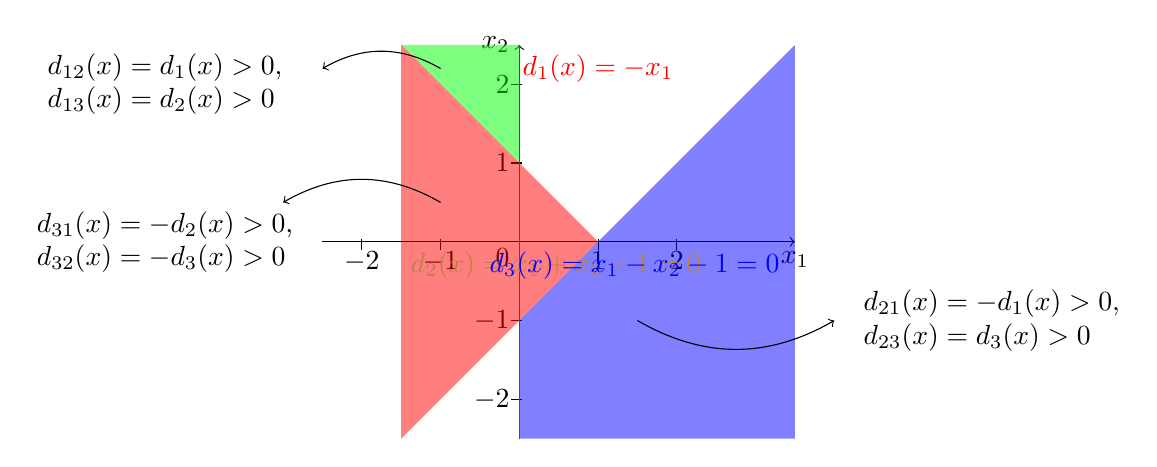
\begin{tikzpicture}  
	 	%axis
	 	\draw[->] (-2.5,0) -- (3.5,0) node[below] {$x_1$};
	 	\draw[->] (0,-2.5) -- (0,2.5) node[left] {$x_2$};
	 	%ticks
	 	\foreach \x in {-2,-1,1,2}
	 	\draw (\x, 1pt) -- (\x, -3pt)
	 	node[below] at (\x,0) {$\x$};
	 	\foreach \y in {-2,-1,1,2}	
	 	\draw (1pt,\y) -- (-3pt,\y)
	 	node [left]at (0,\y) {$\y$}; 
	 	\node [left,yshift = -0.2cm] at(0,0) {$0$};   
	 	%color
	 	\fill[color = green, fill opacity = 0.5] (0,1) -- (0,2.5)   -- (-1.5,2.5) --cycle;
	 	\fill[color = blue, fill opacity = 0.5] (0,-1)-- (3.5,2.5)-- (3.5,-2.5) -- (0,-2.5) --cycle;
	 	\fill[color = red, fill opacity = 0.5] (1,0) -- (-1.5,2.5) -- (-1.5,-2.5) --cycle;	 		 
	 	%draw functions 
	 	%d1
	 	\draw[color = red] (0,-2.5) -- (0,2.5) ;	
	 	\node[color = red] at (1,2.2) {$d_1(x) = -x_1$ };  
	 	%d2
	 	\draw[color = brown,domain = -1.5:3.5] plot[id = x] function{1 - x}
	 	node[below right,xshift = -1.5cm] {$d_2(x) = x_1 + x_2 - 1 = 0$};
	 	%d3
	 	\draw[color = blue, domain = -1.5:3.5] plot[id = x] function{x-1} 
	 	node[below right,xshift = -0.5cm ] {$d_3(x) = x_1 - x_2 -1 = 0$};	
	 	%area 
	 	\path[->] (-1 ,2.2) edge [bend right] node [left] {} (-2.5,2.2);
	 	\node [align = left] at (-4.5,2) { 
	 		$ d_{12}(x) = d_1(x) > 0$,\\
	 		$ d_{13}(x) = d_2(x) > 0$};
	 	%path
	 	\path[->] (1.5, -1) edge [bend right] node [right] {} (4 ,-1);
	 	\node[align = left] at (6,-1) {
	 		$d_{21}(x) = -d_1(x) > 0$,\\
	 		$d_{23}(x) = d_3(x) > 0$ };
	 	%path
	 	\path[->] (-1.0, 0.5) edge [bend right] node [left] {} (-3,0.5);
	 	\node[align = left] at (-4.5,0) {
	 		$ d_{31}(x) = -d_2(x) > 0 $,\\
	 		$ d_{32}(x) = -d_3(x) > 0 $};		
	 	
	 	   	   	
	 	\end{tikzpicture}
	 	\caption{多类情况2的判别界面示意图}
	 \end{figure} 	
	
	\item 多类情况3的条件下,
	 \begin{figure}[H]
	 	\centering 
	 	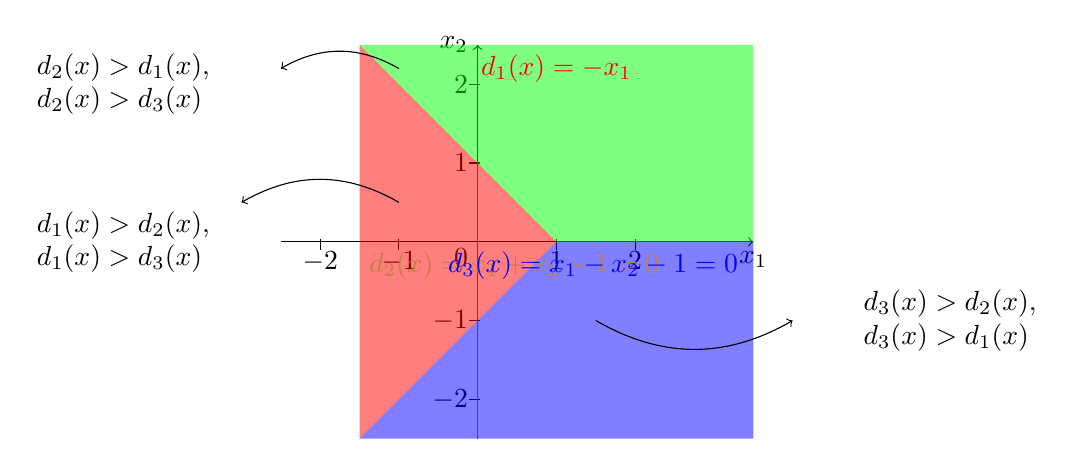
\begin{tikzpicture}  
	 	%axis
	 	\draw[->] (-2.5,0) -- (3.5,0) node[below] {$x_1$};
	 	\draw[->] (0,-2.5) -- (0,2.5) node[left] {$x_2$};
	 	%ticks
	 	\foreach \x in {-2,-1,1,2}
	 	\draw (\x, 1pt) -- (\x, -3pt)
	 	node[below] at (\x,0) {$\x$};
	 	\foreach \y in {-2,-1,1,2}	
	 	\draw (1pt,\y) -- (-3pt,\y)
	 	node [left]at (0,\y) {$\y$}; 
	 	\node [left,yshift = -0.2cm] at(0,0) {$0$};   
	 	%color
	 	\fill[color = green, fill opacity = 0.5]  (-1.5,2.5) -- (1,0) --(3.5,0) -- (3.5,2.5) --cycle;
	 	\fill[color = blue, fill opacity = 0.5]  (1,0)-- (3.5,0)-- (3.5,-2.5) -- (-1.5,-2.5) --cycle;
	 	\fill[color = red, fill opacity = 0.5] (1,0) -- (-1.5,2.5) -- (-1.5,-2.5) --cycle;	 		 
	 	%draw functions 
	 	%d1
	 	\draw[color = red] (0,-2.5) -- (0,2.5) ;	
	 	\node[color = red] at (1,2.2) {$d_1(x) = -x_1$ };  
	 	%d2
	 	\draw[color = brown,domain = -1.5:3.5] plot[id = x] function{1 - x}
	 	node[below right,xshift = -1.5cm] {$d_2(x) = x_1 + x_2 - 1 = 0$};
	 	%d3
	 	\draw[color = blue, domain = -1.5:3.5] plot[id = x] function{x-1} 
	 	node[below right,xshift = -0.5cm ] {$d_3(x) = x_1 - x_2 -1 = 0$};	
	 	%area 
	 	\path[->] (-1 ,2.2) edge [bend right] node [left] {} (-2.5,2.2);
	 	\node [align = left] at (-4.5,2) { 
	 		$ d_2(x) > d_1(x)  $,\\
	 		$ d_2(x) > d_3(x)  $};
	 	%path
	 	\path[->] (1.5, -1) edge [bend right] node [right] {} (4 ,-1);
	 	\node[align = left] at (6,-1) {
	 		$d_3(x) > d_2(x)$,\\
	 		$d_3(x) > d_1(x)$ };
	 	%path
	 	\path[->] (-1.0, 0.5) edge [bend right] node [left] {} (-3,0.5);
	 	\node[align = left] at (-4.5,0) {
	 		$d_1(x) > d_2(x)$,\\
	 		$d_1(x) > d_3(x)$} ;		
	 	
	 	
	 	\end{tikzpicture}
	 	\caption{多类情况3的判别界面示意图}
	 \end{figure} 	
	
	
\end{enumerate}	
	
\section{Problem 3}	
 若数据线性可分,则至少需要 $C_4^1 = 4$个系数分量;若要建立二次的多项式判别
 函数,则至少需要$C_5^2 = 10$个系数分量.
 
 \section{Problem 4}
\textbf{Q: }
用感知器算法求下列模式分类的解向量w:
	\[ \begin{split} 
		 w_1: &{(0,0,0)^T, (1,0, 0)^T, (1, 0, 1)^T, (1, 1, 0)^T} \\
		 w_2: &{(0,0,1)^T, (0,1, 1)^T, (0, 1, 0)^T, (1, 1, 1)^T} \\
		\end{split}  
	\]
\textbf{A: }
 二分类的感知机算法训练过程如下:
  \begin{itemize}
  	\item 线性分类器设为$h_{\bm{w}}(\bm{x}) = \text{sign}(\bm{w}^T\bm{x} + b)$, $\text{sign}$为符号函数 ,
	  	如果 $\bm{w}^T\bm{x} + b \geq 0 $ 那么$h = 1$否则$h = -1$;
	\item 分类损失loss定义为分类错误加$1$,分类正确不变; 
	\item 扩充每个样本$\bm{x}$ 为$[\bm{x},1]$的向量,参数设为$\bm{\theta} = [\bm{w}, b]$, 参数更新规则:
		\[
			\bm{\theta}_j = \bm{\theta}_j + \alpha (y^{(i)} - h_{\bm{\theta}}(x^{(i)}))\bm{x}_j^{(i)}, i= 1,2,...,m, j=1,2,...,n
		\]
		其中$m$为样本数量, $n$为参数的维度, $\alpha$为学习速率.
	\item 初始化参数进行迭代, 当总的分类损失为0就停止训练得到一个线性分类器, 若loss不能降为0则表明有的样本未分类正确,
		数据不是线性可分.
  \end{itemize}
  程序及测试结果如下
 \inputpython{perceptron.py}{1}{70}
  测试结果:   
  \begin{figure}[H]
  	\centering
  	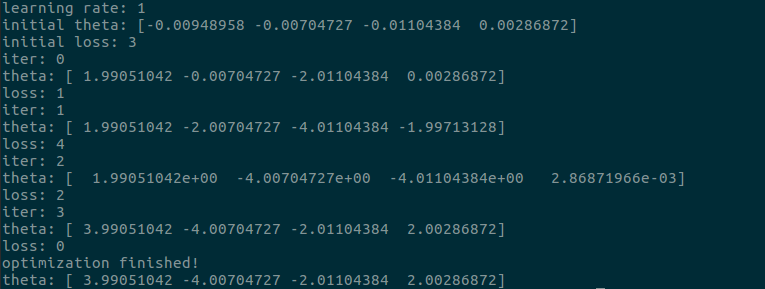
\includegraphics[width = 0.9\textwidth]{result}
  \end{figure}
  $3$次迭代得到一个参数$\theta = [3.99051042 ,-4.00704727, -2.01104384,  2.00286872]$,判别函数
  \[
	  D(x) = 3.99051042x_1 -4.00704727x_2 -2.01104384x_3 +  2.00286872
  \]
\section{Problem 5}
\textbf{Q: }
用多类感知器算法求下列模式的判别函数:
\[
 \begin{split} 
	w_1: & (-1,-1)^T\\
	w_2: & (0,0)^T \\
	w_3: & (1,1)^T 
 \end{split}  
\]
\textbf{A: } \\
 依次选取一类样本作为正样本,其余作为负样本,进行二分类的感知机训练,得到3个判别函数.
  程序及测试结果如下
  \inputpython{multi_class.py}{1}{70}
  测试结果:   
  \begin{figure}[H]
  	\centering
  	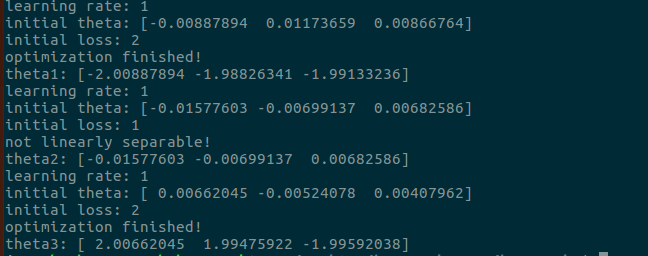
\includegraphics[width = 0.9\textwidth]{multi}
  \end{figure}	
 对于类别$w_1$, 线性可分,一个判别函数为
 \[
	 d_1(x) = -2.00887894x_1 -1.98826341x_2 -1.99133236
 \]	
 对于类别$w_2$, 线性不可分, 判别函数
 \[
	 d_2(x) = 0
 \]
 对于类别$w_3$, 线性可分, 一个判别函数
 \[
     d_3(x) = 2.00662045x_1 +1.99475922x_2 -1.99592038
 \]
\section{Problem 4}
 \textbf{Q: }
采用梯度法和准则函数 
\[
	J(w,x,b) = \frac{1}{8||x||^2} [(w^Tx - b) - |w^Tx-b|]^2
\]
式中实数b>0,试导出两类模式的分类算法。 \\
 \textbf{A: }
\[
   J(w,x,b) =  \left\lbrace
     \begin{split}
        0, &\text{ if } w^Tx - b > 0 \\
         \frac{1}{2||x||^2}(w^Tx - b)^2, &\text{ otherwise}
     \end{split}
   \right. 
\]
 $J$对$w$求导得
 \[
   \frac{\partial J}{\partial w} = \left\lbrace 
     \begin{split}
	     0, &\text{ if } w^Tx - b > 0 \\ 
	     \frac{1}{||x||^2}(w^Tx - b)x, &\text{ otherwise}
     \end{split}
    \right.  
 \]
 对$b$求导,得
 \[
    \frac{\partial J}{\partial b} = \left\lbrace 
    \begin{split}
    0, &\text{ if } w^Tx - b > 0 \\ 
    -\frac{1}{||x||^2}(w^Tx - b), &\text{ otherwise}
    \end{split}
    \right.  
 \]
 参数更新规则
 \begin{itemize}
 	\item 初始化$w$,$b$
 	\item 选取一个样本$x$, 计算$h = w^Tx-b$, 若$h > 0$ 则参数不变,继续选取一个样本;
 	否则, 计算梯度,更新参数:
 	  \[ \begin{split} 
    	    w := &w + \alpha \frac{1}{||x||^2}(b-w^Tx)x, \\
    	    b := &b + \alpha\frac{1}{||x||^2}(w^Tx - b) ,\alpha > 0
    	 \end{split} 
 	  \]
 	\item 如果模式线性可分,则当所有样本均满足 $w^Tx - b > 0$时停止训练;否则得不到收敛结果.
 \end{itemize}
 
\section{Problem 5} 
\textbf{Q: } 用二次埃尔米特多项式的势函数算法求解以下模式的分类问题 
   \[  \begin{split} 
 		w_1: {(0, 1)^T, (0, -1)^T} \\
		w_2: {(1, 0)^T, (-1, 0)^T}
	  \end{split} 	
	\]
\textbf{A: } \\
选择Hermite 多项式,其正交域为$(-\infty,+\infty)$,其一维形式为
\[ \begin{split} 
	\varphi_k &=  \frac{\exp(-x^2/2)}{\sqrt{2^k\cdot k!\sqrt{\pi}}}H_k(x) , k = 0,1,2... \\
	H_n(x) &= (-1)^n \exp(x^2) \frac{\mathrm{d}^n}{\mathrm{d}x^n}\exp(-x^2)
   \end{split} 		
\]
其正交性
\[
	\int_{-\infty}^{\infty} H_m(x)H_n(x) \exp(-x^2)\mathrm{d}x = \left\lbrace
	 \begin{split}
		 0, & m\neq n\\
		 2^n n!\sqrt{\pi}, & m = n
	 \end{split}
	\right. 
\]
其中,$H_k(x)$前面的乘式为正交归一化因子,为计算简便可省略。因此,Hermite多项式前面几项的表达式为 
\[ \begin{split} 
		H_0(x) &= 1, H_1(x) = 2x, H_2(x) = 4x^2 - 2, \\
		H_3(x) &= 8x^3 - 12x, H_4(x)  = 16x^4 - 48x^2 + 12
	\end{split} 
\]
建立二维的正交函数集,这里取$9$项最低阶的二维的正交函数
\[ \begin{split} 
	\varphi_1(x) &= \varphi_1(x_1,x_2) = H_0(x_1)H_0(x_2) = 1 \\
	\varphi_2(x) &= \varphi_2(x_1,x_2) = H_1(x_1)H_0(x_2) = 2x_1 \\
	\varphi_3(x) &= \varphi_3(x_1,x_2) = H_0(x_1)H_1(x_2) = 2x_2 \\
	\varphi_4(x) &= \varphi_4(x_1,x_2) = H_1(x_1)H_1(x_2) = 4x_1x_2 \\
	\varphi_5(x) &= \varphi_5(x_1,x_2) = H_0(x_1)H_2(x_2) = 4x_2^2 - 2 \\
	\varphi_6(x) &= \varphi_6(x_1,x_2) = H_1(x_1)H_2(x_2) = 2x_1(4x_2^2-2)  \\	
	\varphi_7(x) &= \varphi_7(x_1,x_2) = H_2(x_1)H_0(x_2) = 4x_1^2 - 2\\
	\varphi_8(x) &= \varphi_8(x_1,x_2) = H_2(x_1)H_1(x_2) = (4x_2^2 - 2)2x_2 \\
	\varphi_9(x) &= \varphi_9(x_1,x_2) = H_2(x_1)H_2(x_2) = (4x_1^2 - 2)(4x_2^2 - 2) \\
 \end{split} 
\]
按第一类势函数的定义生成势函数,
\[
	K(x,x_k) = \sum_{i=1}^{9}\varphi_i(x)\varphi_i(x_k)  
\]
\[
 d(x) = -32x_1^2+32x_2^2
\] 
\section{Problem 6}
\[
\begin{split}
  K(x,x_k) &= e^{-\alpha[(x_1-x_{k1})^2+(x_2-x_{k2})^2]} \\
  d(x) &= e^{-\alpha}[e^{-x_1^2-(x_2+1)^2} + e^{-x_1^2-(x_2-1)^2} - e^{-(x_1-1)^2-x_2^2}-e^{-(x_1+1)^2-x_2^2}]
\end{split}
\]




\end{document}